\chapter{Differential Equations}

\section{Definitions}

\begin{definition}
    A \vocab{differential equation} (DE) is an equation which involves one or more derivatives of a function $y$ with respect to a variable $x$ (i.e. $y'$, $y''$, etc.). The \vocab{order} of a differential equation is determined by the highest derivative in the equation. The \vocab{degree} of a differential equation is the power of the highest derivative in the equation.
\end{definition}

\begin{example}[Order and Degree]
    The differential equation \[x \bp{\der[2]{y}{x}}^3 + x^2 \bp{\der{y}{x}} + y = 0\] has order 2 and degree 3.
\end{example}

\begin{definition}
    The \vocab{general solution} represents the full family of solutions to a differential equation. A \vocab{particular solution} is a specific member of the family of solutions.
\end{definition}

\begin{example}
    The differential equation $y' = 2x$ has general solution $y = x^2 + C$, where $C$ is an arbitrary constant. Any member of this family, such as $y = x^2$, $y = x^2 + 2$ or $y = x^2 - 10$, are particular solutions to $y' = 2x$.  
\end{example}

In general, the general solution of an $n$th order differential equation has $n$ arbitrary constants.

\section{Solving Differential Equations}

In this section, we introduce methods to solve three special types of differential equations, namely
\begin{itemize}
    \item separable differential equation,
    \item first-order linear differential equation, and
    \item second-order linear differential equation with constant coefficients.
\end{itemize}
We also demonstrate how to solve differential equations using a given substitution, which is useful if the differential equation to be solved is not in one of the above three forms.

\subsection{Separable Differential Equation}

\begin{definition}
    A \vocab{separable differential equation} is a differential equation that can be written in the form \[\der{y}{x} = f(x) g(y).\]
\end{definition}

\begin{recipe}[Solving via Separation of Variables]
    \phantom{.}
    \begin{enumerate}
        \item Separate the variables. \[\frac1{g(y)} \der{y}{x} = f(x).\]
        \item Integrate both sides with respect to $x$. \[\int \frac1{g(y)} \der{y}{x} \d x = \int f(x) \d x.\]
        \item Simplify the LHS. \[\int \frac1{g(y)} \d y = \int f(x) \d x.\]
        \item Evaluate both integrals.
    \end{enumerate}
\end{recipe}

\begin{sample}
    Find the general solution to \[2x \der{y}{x} = y^2 + 1.\]
\end{sample}
\begin{sampans}
    Separating variables, \[\frac2{y^2 + 1} \der{y}{x} = \frac1{x}.\] Integrating both sides with respect to $x$, we get \[\int \frac2{y^2 + 1} \der{y}{x} \d x = \int \frac1{x} \d x.\] The LHS simplifies to \[\int \frac2{y^2 + 1} \d y = \int \frac1{x} \d x.\] Evaluating the two integrals, we have $2\arctan y = \ln \abs{x} + C$. This is the general solution to the given differential equation.
\end{sampans}

\subsection{First-Order Linear Differential Equation}

\begin{definition}
    A \vocab{first-order linear differential equation} is a differential equation that can be written in the form \[\der{y}{x} + p(x) \, y = q(x).\]
\end{definition}

To solve a linear first-order differential equation, we first observe that the LHS looks like the product rule has been applied. This motivates us to multiply through by a new function $f(x)$ such that the LHS can be written as the derivative of a product: \[f(x) \der{y}{x} + f(x) \, p(x) \, y = f(x) \, q(x). \tag{$\ast$}\] Comparing \[\der{}{x} \bs{f(x) \, y} = f(x) \der{y}{x} + f'(x) \, y,\] with the LHS of ($\ast$), we require $f(x) \, p(x) = f'(x)$.

We now solve for $f(x)$. Since \[\frac{f'(x)}{f(x)} = p(x),\] we may integrate both sides with respect to $x$ to get \[\ln f(x) = \int p(x) \d x,\] so $f(x) = \e^{\int p(x) \d x}$.

Substituting this back in ($\ast$), we have \[\der{}{x} \bs{y \e^{\int p(x) \d x}} = q(x) \e^{\int p(x) \d x}.\] Integrating both sides with respect to $x$, we find that \[y \e^{\int p(x) \d x} = \int q(x) \e^{\int p(x) \d x} \d x.\] This is the general solution to the differential equation.

\begin{definition}
    The function $f(x) = \e^{\int p(x) \d x}$ is called the \vocab{integrating factor}, sometimes denoted ``$\IF$''.
\end{definition}

When finding the integrating factor, we do not need to include the arbitrary constant or consider absolute values, as they will simplify to the same result anyway.

\begin{recipe}[Solving via Integrating Factor]
    \phantom{.}
    \begin{enumerate}
        \item Multiply the differential equation through by the $\IF = \e^{\int p(x) \d x}$. \[\e^{\int p(x) \d x} \der{y}{x} + \e^{\int p(x) \d x} p(x) y = \e^{\int p(x) \d x} q(x).\]
        \item Express the LHS as the derivative of a product. \[\der{}{x} \bs{y \e^{\int p(x) \d x}} = \e^{\int p(x) \d x} q(x).\]
        \item Integrate both sides with respect to $x$. \[y \e^{\int p(x) \d x} = \int \e^{\int p(x) \d x} q(x) \d x.\]
    \end{enumerate}
\end{recipe}

\begin{sample}
    Find the general solution to \[x \der{y}{x} + 3y = 5x^2.\]
\end{sample}
\begin{sampans}
    Writing the given differential equation in standard form, we have \[\der{y}{x} + \bp{\frac3x}y = 5x.\] The integrating factor is hence \[\IF = \e^{\int 3/x \d x} = \e^{3\ln x} = x^3.\] Multiplying the integrating factor through the differential equation, we see that \[\der{}{x} \bp{x^3 y} = x^3 \der{y}{x} + 3x^2 y = 5x^4.\] Integrating the extreme left and right sides with respect to $x$, we get\[x^3 y = \int 5x^4 \d x = x^5 + C.\] Thus, the general solution is $y = x^2 + Cx^{-3}$.
\end{sampans}

\subsection{Second-Order Linear Differential Equations with Constant Coefficients}

In this section, we look at second-order linear differential equations and constant coefficients, which has the general form \[a \der[2]{y}{x} + b \der{y}{x} + cy = f(x).\] If $f(x) \equiv 0$, we call the differential equation \vocab{homogeneous}. Else, it is \vocab{non-homogeneous}. In general, a second-order differential equation will have two solutions.

Before looking at the methods to solve second-order differential equations, we introduce two important concepts, namely the superposition principle and linear independence.

\begin{theorem}[Superposition Principle]
    Let $y_1$ and $y_2$ be solutions to a linear, homogeneous differential equation. Then $A y_1 + B y_2$ is also a solution to the differential equation.
\end{theorem}
\begin{proof}
    We consider the case where the differential equation has order 2, though the proof easily generalizes to higher orders.

    Suppose $y_1$ and $y_2$ are solutions to \[a \der[2]{y}{x} + b \der{y}{x} + c y = 0.\] Substituting $y = A y_1 + B y_2$ into the differential equation, we get
    \begin{align*}
        &a \bp{A y_1'' + By_2''} + b \bp{A y_1' + By_2'} + c\bp{Ay_1 + By_2}\\
        &\hspace{2em}= A\bp{ay_1'' + by_1' + cy_1} + B\bp{ay_2'' + by_2' + cy_2}\\
        &\hspace{2em}= 0.
    \end{align*}
    Hence, $A y_1 + By_2$ satisfies the differential equation and is hence a solution.
\end{proof}

\begin{definition}
    Two functions $y_1$ and $y_2$ are \vocab{linearly independent} if the only solution to $A y_1 + B y_2 = 0$ is the trivial solution $A = B = 0$. If there exists non-zero solutions to $A$ and $B$, then the two functions are \vocab{linearly dependent}.
\end{definition}

We are now ready to solve second-order differential equations.

\subsubsection{Homogeneous Second-Order Linear Differential Equations with Constant Coefficients}

A homogeneous \emph{first}-order linear differential equation with constant coefficients \[a \der{y}{x} + by = 0\] has the general solution $y = C \e^{-bx/a}$.

This motivates us to look for exponential solutions to the second-order case. That is, we suppose that $y= \e^{mx}$ is a solution to \[a \der[2]{y}{x} + b \der{y}{x} + cy = 0,\] where $m$ is a constant to be determined. Substituting $y = \e^{mx}$ into the differential equation, we get $am^2 \e^{mx} + bm \e^{mx} + c\e^{mx} = 0$. Dividing by $\e^{mx}$, we get the quadratic $am^2 + bm + c = 0$. This is known as the \vocab{characteristic equation} of the differential equation.

By solving the characteristic equation for $m$, we can recover the solutions to the differential equation. Since the characteristic equation is quadratic, it has, in general, two roots, say $m_1$ and $m_2$. We then have the following three scenarios to consider:
\begin{itemize}
    \item The roots are real and distinct.
    \item The roots are real and equal.
    \item The roots are complex conjugates.
\end{itemize}

\paragraph{Real and Distinct Roots.} If $m_1$ and $m_2$ are real and distinct, both $y_1 = \e^{m_1 x}$ and $y_2 = \e^{m_2 x}$ are solutions to the differential equation. Hence, by the superposition principle, the general solution is $y = A \e^{m_1 x} + B \e^{m_2 x}$, where $A$ and $B$ are constants.

\paragraph{Real and Equal Roots.} If the two roots are equal, i.e. $m_1 = m_2 = m$, then $y_1 = \e^{m_1 x}$ and $y_2 = \e^{m_2 x}$ are no longer linearly independent. That is, we only recover one solution $y_1 = \e^{mx}$. We thus have to find another solution that is not a constant multiple of $\e^{mx}$. By intelligently guessing a solution, we see that $y_2 = x \e^{mx}$ satisfies the differential equation. Hence, by the superposition principle, the general solution is $y = A \e^{mx} + Bx \e^{mx} = (A + Bx) \e^{mx}$.

\paragraph{Complex Roots.} If the two roots are complex, then they are conjugates, and we can write them as $m_1 = p + \i q$ and $m_2 = p - \i q$. Then \[y_1 = \e^{(p + \i q)x} = \e^{px} \bp{\cos qx + \i \sin qx} \quad \tand \quad y_2 = \e^{(p -\i q) x} = \e^{px} \bp{\cos qx - \i \sin qx}.\] By the superposition principle, we get the general solution
\begin{align*}
    y &= C\e^{px} \bp{\cos qx + \i \sin qx} + D\e^{px} \bp{\cos qx - \i \sin qx}\\
    &= \e^{px} \bp{A \cos qx + B \sin qx},
\end{align*}
where $A = C + D$ and $B = \i (C - D)$ are arbitrary constants.

In summary,
\begin{recipe}[Solving a Homogeneous Second-Order Linear Differential Equation with Constant Coefficients]
    To solve the second-order differential equation \[a \der[2]{y}{x} + b \der{y}{x} + cy = 0,\]
    \begin{enumerate}
        \item Form the characteristic equation $am^2 + bm + c = 0$.
        \item Find the roots $m_1$ and $m_2$ of this characteristic equation.
        \item \begin{itemize}
            \item If $m_1$ and $m_2$ are real and distinct, then $y = A \e^{m_1 x} + B \e^{m_2 x}$.
            \item If $m_1$ and $m_2$ are real and equal, i.e. $m_1 = m_2 = m$, then $y = (A + Bx) \e^{m x}$.
            \item If $m_1$ and $m_2$ are complex, i.e. $m_1 = p + \i q$ and $m_2 = p - \i q$, then $y = \e^{px} \bp{A \cos qx + B \sin qx}$.
        \end{itemize}
    \end{enumerate}    
\end{recipe}

\subsubsection{Non-Homogeneous Second-Order Linear Differential Equations with Constant Coefficients}

We now consider the non-homogeneous second-order linear differential equation with constant coefficients, which takes the form \[a \der[2]{y}{x} + b \der{y}{x} + c y = f(x).\] In order to solve this differential equation, we apply the following result:

\begin{theorem}
    The general solution to \[a \der[2]{y}{x} + b \der{y}{x} + c y = f(x) \tag{$\ast$}\] is $y = y_c + y_p$, where $y_p$ is a particular solution to ($\ast$), and $y_c$ is the general solution to the associated differential equation \[a \der[2]{y}{x} + b \der{y}{x} + c y = 0.\]
\end{theorem}
\begin{proof}
    Since $y_p$ is a particular solution to ($\ast$), we have \[a \der[2]{y}{x} + b \der{y}{x} + c y = f(x) \quad \tand \quad a \der[2]{y_p}{x} + b \der{y_p}{x} + c y_p = f(x).\] Subtracting, we see that \[a \der[2]{}{x} \bp{y - y_p} + b \der{}{x} \bp{y - y_p} + c\bp{y - y_p} = 0.\] That is, $y - y_p$ is a solution to the associated differential equation. Thus, $y - y_p = y_c$, giving $y = y_c + y_p$ as desired.
\end{proof}

Note that $y_c$ is called the \vocab{complementary solution} while $y_p$ is called the \vocab{particular integral} or \vocab{particular solution}.

As we know how to solve the homogeneous differential equation, obtaining $y_c$ is easy. The hard part is finding a particular solution $y_p$. However, if we make some intelligent guesses, we can determine the general form of $y_p$. This is called the \vocab{method of undetermined coefficients}. We demonstrate this method with the following example:

\begin{example}[Method of Undetermined Coefficients]
    Consider the differential equation \[\der[2]{y}{x} + 3\der{y}{x} - 4y = 3 + 8x^2.\] The complementary solution $y_c$ is easily found to be $y_c = A\e^x + B\e^{-4x}$.
    
    Observing $3 + 8x^2$ to be a polynomial of degree 2, we guess that the particular solution  $y_p$ is also a polynomial of degree 2, i.e. $y_p = Cx^2 + Dx + E$, for some coefficients $C$, $D$ and $E$ to be determined (hence the name ``method of undetermined coefficients''). Substituting this into the differential equation yields \[\bp{2C} + 3\bp{2Cx + D} - 4\bp{Cx^2 + Dx + E} = 3 + 8x^2.\] Comparing coefficients, we get the system \[\systeme[CDE]{-4C = 8,6C-4D = 0,2C + 3D - 4E = 3},\] whence $C = -2$, $D = -3$ and $E = -4$. Thus, the particular solution is $y_p = -2x^2 - 3x - 4$ and the general solution is $y = y_c + y_p = A\e^x + B\e^{-4x} - 2x^2 - 3x - 4$.
\end{example}

In our syllabus, we are only required to solve non-homogeneous differential equations where $f(x)$ is a polynomial of degree $n$ (as above), of the form $p\e^{kx}$, or of the form $p\cos kx + q\sin kx$. The ``guess'' for $y_p$ in each of the three cases is tabulated below:

\begin{table}[H]
    \centering
    \begin{tabular}{|c|c|}
    \hline
    $f(x)$ & \bd{``Guess'' for $y_p$} \\ \hline\hline
    Polynomial of degree $n$ & Polynomial of degree $n$ \\ \hline
    $p\e^{kx}$ & $C \e^{kx}$ \\ \hline
    $p \cos kx + q \sin kx$ & $C \cos kx + D \sin kx$ \\ \hline
    \end{tabular}
    \caption{}
\end{table}

In the event where our ``guess'' for $y_p$ appears in the complementary function $y_c$, we need to make some adjustments to our ``guess'' (similar to the case where $m_1 = m_2$ when solving a homogeneous differential equation). Typically, we multiply the guess by powers $x$ until the guess no longer appears in the complementary function.

\begin{example}[Adjusting $y_p$]
    \phantom{.}
    \begin{itemize}
        \item If $a y'' + by' + cy = \e^{2x}$ has complementary function $y_c = A\e^{-5x} + B\e^{2x}$, we try $y_p = Cx\e^{2x}$.
        \item If $a y'' + by' + cy = \e^{2x}$ has complementary function $y_c = (A + Bx) \e^{2x}$, we try $y_p = Cx^2\e^{2x}$.
    \end{itemize}
\end{example}

\subsection{Solving via Substitution}

Sometimes, we are given a differential equation that is not of the forms described in this section. We must then use the given substitution function to simplify the original differential equation into one of the standard forms. Similar to integration by substitution, all instances of the dependent variable (including its derivatives) must be substituted.

\begin{recipe}[Solving via Substitution]
    \phantom{.}
    \begin{enumerate}
        \item Differentiate the given substitution function.
        \item Substitute into the original differential equation and simplify to obtain another differential equation that we know how to solve.
        \item Obtain the general solution of the new differential equation with new dependent variables.
        \item Express the solution in terms of the original variables.
    \end{enumerate}
\end{recipe}

\begin{sample}
    By using the substitution $y = ux^2$, find the general solution of the differential equation \[x^2 \der{y}{x} - 2xy = y^2, \quad x > 0.\]
\end{sample}
\begin{sampans}
    From $y = ux^2$, we see that \[\der{y}{x} = 2ux + x^2 \der{u}{x}.\] Substituting this into the original differential equation, \[x^2 \bp{2ux + x^2 \der{u}{x}} - 2x \bp{ux^2} = \bp{ux^2}^2.\] Simplifying, we get the separable differential equation \[\der{u}{x} = u^2,\] which we can easily solve: \[-\frac1u = \int \frac1{u^2} \d u = \int 1 \d x = x + C.\] Re-substituting $y$ back in, we have the general solution \[-\frac{x^2}{y} = x + C.\]
\end{sampans}

\section{Family of Solution Curves}

Graphically, the general solution of a differential equation is represented by a family of solution curves which contains infinitely many curves as the arbitrary constant $c$ can take any real number.

A particular solution of the differential equation is represented graphically by one member of that family of solution curves (i.e. one value of the arbitrary constant).

When sketching a family of curves, we choose values of the arbitrary constant that will result in qualitatively different curves. We also need to sketch sufficient members (usually at least 3) of the family to show all the general features of the family.

\begin{example}[Sketch of Family of Solution Curves]
    The following diagram shows three members of the family of solution curves for the general solution $y = A\e^{x^2}$.

    \begin{figure}[H]\tikzsetnextfilename{370}
        \centering
        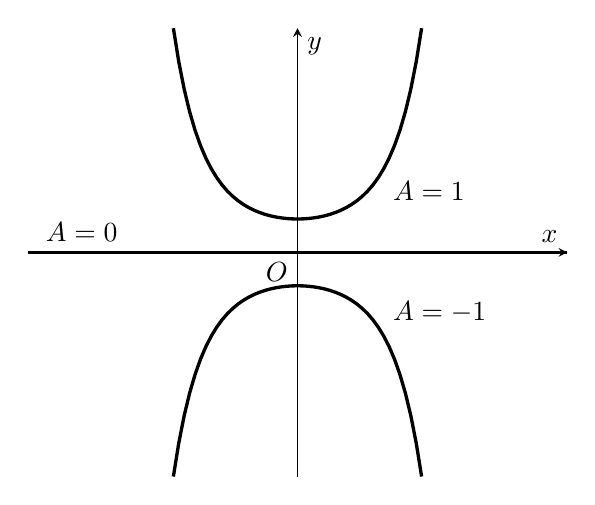
\begin{tikzpicture}[trim axis left, trim axis right]
            \begin{axis}[
                domain = -3:3,
                restrict y to domain =-7:7,
                samples = 101,
                axis y line=middle,
                axis x line=middle,
                xtick = \empty,
                ytick = \empty,
                xlabel = {$x$},
                ylabel = {$y$},
                legend cell align={left},
                legend pos=outer north east,
                after end axis/.code={
                    \path (axis cs:0,0) 
                        node [anchor=north east] {$O$};
                    }
                ]
                \addplot[very thick] {e^(x^2)} node[pos=0.65, below right] {$A = 1$};
                \addplot[very thick] {0} node[pos=0.1, above] {$A = 0$};
                \addplot[very thick] {-e^(x^2)} node[pos=0.65, above right] {$A = -1$};
                \end{axis}
        \end{tikzpicture}
        \caption{}
    \end{figure}

    In this example, the shape of the curve depends on the sign of $A$. Thus, to fully represent the family of curves, we must provide sketches of (at least) three members: one where $A > 0$, one where $A = 0$, and one where $A < 0$.
\end{example}

\section{Approximating Solutions}

Most of the time, a first-order differential equation of the general form $\derx{y}{x} = f(x, y)$ cannot be solved exactly and explicitly by analytical methods like those discussed in the earlier sections. In such cases, we can use numerical methods to approximate solutions to differential equations.

Different methods can be used to approximate solutions to a differential equation. A sequence of values $\bc{y_i}$ is generated to approximate the exact solutions at the points $\bc{x_i}$. It must be emphasized that the numerical methods do not generate a formula for the solution to the differential equation. Rather, they generate a sequence of approximations to the actual solution at the specified points.

In this section, we look at Euler's Method, as well as the improved Euler's Method.

\subsection{Euler's Method}

The key principle in Euler's method is the use of a linear approximation for the tangent line to the actual solution curve $y(t)$ to approximate a solution.

\begin{recipe}[Euler's Method]
    Given an initial value problem \[\der{y}{t} = f(t, y), \quad y(t_0) = y_0,\] Euler's method,  with step size $\D t$, uses the recurrence relation $y_{n} = y_{n-1} + \D t \, f(t_{n-1}, y_{n-1})$ to approximate $y(t_n) \approx y_n$.
\end{recipe}

\begin{figure}[H]\tikzsetnextfilename{371}
    \centering
    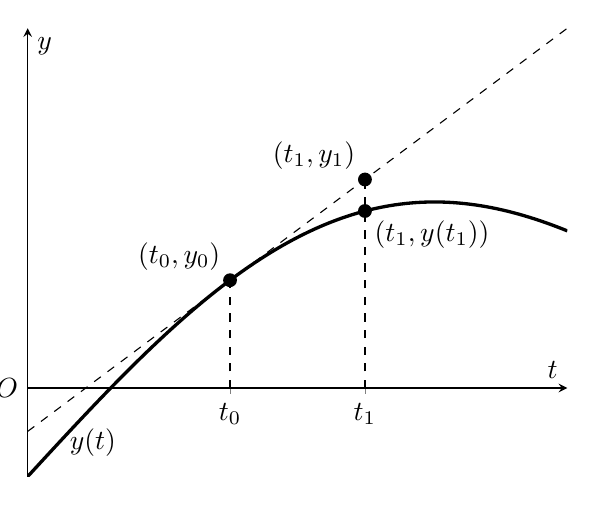
\begin{tikzpicture}[trim axis left, trim axis right]
        \begin{axis}[
            domain = 0:0.8,
            samples = 101,
            axis y line=middle,
            axis x line=middle,
            xtick = {0.3, 0.5},
            xticklabels = {$t_0$, $t_1$},
            ytick = \empty,
            xlabel = {$t$},
            ylabel = {$y$},
            legend cell align={left},
            legend pos=outer north east,
            after end axis/.code={
                \path (axis cs:0,0) 
                    node [anchor=east] {$O$};
                }
            ]
            \addplot[very thick] {x + sin(pi * \x r) - 0.5} node[pos=0.1, right] {$y(t)$};

            \addplot[dashed] {0.609 + 2.847 * (x - 0.3)};
            \draw[dashed] (0.3, 0) -- (0.3, 0.609);
            \draw[dashed] (0.5, 0) -- (0.5, 1.178);
            \fill (0.5, 1.178) circle[radius=2.5pt] node[anchor=south east] {$(t_1, y_1)$};
            \fill (0.3, 0.609) circle[radius=2.5pt] node[anchor=south east] {$(t_0, y_0)$};
            \fill (0.5, 1) circle[radius=2.5pt] node[anchor=north west] {$(t_1, y(t_1))$};
            \end{axis}
    \end{tikzpicture}
    \caption{}
\end{figure}

To derive Euler's method, we begin at $(t_0, y_0)$ on the solution curve. Here, the gradient of the curve is $f(t_0, y_0)$. Hence, by the point-slope formula, the equation of the tangent line through $(t_0, y_0)$ is $y - y_0 = (t - t_0) f(t_0, y_0)$. For values of $t$ near $t_0$, the tangent line approximates the solution curve. In particular, choosing $t = t_1 = t_0 + \D t$, we have that $y(t_1) \approx y_1 = y_0 + \D t \, f(t_0, y_0)$. Repeating this process, we have in general that $y_{n} = y_{n-1} + \D t \, f(t_{n-1}, y_{n-1})$. This is Euler's method.

\begin{example}[Euler's Method]\label{eg:Eulers-Method}
    Consider the initial value problem \[\der{y}{t} = 2y - 1, \quad y(0) = \frac32,\] which can be verified to have solution $y = \e^{2t} + 1/2$. Suppose we wish to approximate the value of $y(0.3)$ (which we know to be $\e^{2(0.3)} + 1/2 = 2.322$). Using Euler's method with step size $\D t = 0.1$, we get
    \begin{align*}
        y_1 &= y_0 + \D t \bp{2y_0 - 1} = 1.5 + 0.1 \bs{2(1.5) - 1} = 1.7\\
        y_2 &= y_1 + \D t \bp{2y_1 - 1} = 1.7 + 0.1 \bs{2(1.7) - 1} = 1.94\\
        y_3 &= y_2 + \D t \bp{2y_2 - 1} = 1.94 + 0.1 \bs{2(1.94) - 1} = 2.228
    \end{align*}
    Hence, $y(0.3) \approx y_3 = 2.228$, which is a decent approximation (4.04\% error).
\end{example}

\subsubsection{Error in Approximations}

Similar to the trapezium rule, the nature of the estimates given by Euler's method depends on the concavity of the actual solution curve.
\begin{itemize}
    \item If the actual solution curve is concave upwards (i.e. lies above its tangents), the approximations are under-estimates.
    \item If the actual solution curve is concave downwards (i.e. lies below its tangents), the approximations are over-estimates.
\end{itemize}

Also note that the smaller the step size $\D t$, the better the approximations. However, in doing so, more calculations must be made. This is a situation that is typically of numerical methods: there is a trade-off between accuracy and speed.

\subsection{Improved Euler's Method}

In the previous section, we saw how Euler's method over- or under-estimates the actual solution curve due to the curve's concavity. The improved Euler's method address this.

\begin{recipe}[Improved Euler's Method]
    Given an initial value problem \[\der{y}{t} = f(t, y), \quad y(t_0) = y_0,\] the improved Euler's method, with step size $\D t$, uses the recurrence relation \[y_{n} = y_{n-1} + \D t \bs{\frac{f(t_{n-1}, y_{n-1}) + f(t_{n}, \wt{y}_{n})}{2}},\] where $\wt{y}_{n} = y_{n-1} + \D t \, f(t_{n-1}, y_{n-1})$, to approximate $y(t_n) \approx y_n$.
\end{recipe}

\begin{definition}
    $\wt{y}_{n}$ is called the \vocab{predictor}, while $y_{n}$ is called the \vocab{corrector}.
\end{definition}

We now derive the improved Euler's method. Suppose the actual solution curve is concave upward (the concave downward case is derived identically). Let $T_0$ and $T_1$ be the tangent lines at $t = t_0$ and $t = t_1$, with gradients $m_0$ and $m_1$, respectively. Let $m$ be the gradient of the line passing through both $(t_0, y(t_0))$ and $(t_1, y(t_1))$. We aim to find an approximation to $m$ using only the information we know.

\noindent\begin{minipage}{0.5\textwidth}
\begin{figure}[H]\tikzsetnextfilename{372}
    \centering
    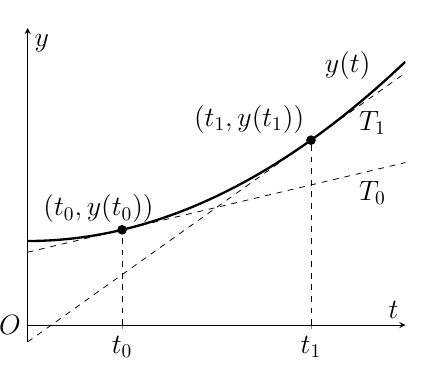
\begin{tikzpicture}[trim axis left, trim axis right, scale=0.7]
        \begin{axis}[
            every axis/.append style={font=\Large},
            domain = 0:0.8,
            samples = 101,
            ymax=1.06,
            axis y line=middle,
            axis x line=middle,
            xtick = {0.2, 0.6},
            xticklabels = {$t_0$, $t_1$},
            ytick = \empty,
            xlabel = {$t$},
            ylabel = {$y$},
            legend cell align={left},
            legend pos=outer north east,
            after end axis/.code={
                \path (axis cs:0,0) 
                    node [anchor=east] {$O$};
                }
            ]
            \addplot[very thick] {x^2 + 0.3} node[pos=0.9, above left] {\Large$y(t)$};

            \addplot[dashed] {0.34 + (x - 0.2) * 0.4};
            \addplot[dashed] {0.66 + (x - 0.6) * 1.2};

            \draw[dashed] (0.2, 0) -- (0.2, 0.34);
            \draw[dashed] (0.6, 0) -- (0.6, 0.66);

            \fill (0.2, 0.34) circle[radius=2.5pt];
            \fill (0.6, 0.66) circle[radius=2.5pt] node[anchor=south east] {\Large$(t_1, y(t_1))$};

            \node[anchor=south] at (0.15, 0.34) {\Large$(t_0, y(t_0))$};

            \node at (0.73, 0.72) {\Large$T_1$};
            \node at (0.73, 0.47) {\Large$T_0$};
            \end{axis}
    \end{tikzpicture}
    \caption{\label{fig:de-1}}
\end{figure}
\end{minipage}
\begin{minipage}{0.5\textwidth}
\begin{figure}[H]\tikzsetnextfilename{373}
    \centering
    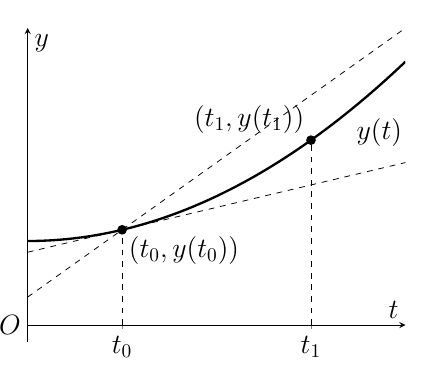
\begin{tikzpicture}[trim axis left, trim axis right, scale=0.7]
        \begin{axis}[
            every axis/.append style={font=\Large},
            domain = 0:0.8,
            samples = 101,
            ymin=-0.06,
            axis y line=middle,
            axis x line=middle,
            xtick = {0.2, 0.6},
            xticklabels = {$t_0$, $t_1$},
            ytick = \empty,
            xlabel = {$t$},
            ylabel = {$y$},
            legend cell align={left},
            legend pos=outer north east,
            after end axis/.code={
                \path (axis cs:0,0) 
                    node [anchor=east] {$O$};
                }
            ]
            \addplot[very thick] {x^2 + 0.3} node[pos=0.8, below right] {\Large$y(t)$};

            \addplot[dashed] {0.34 + (x - 0.2) * 0.4};
            \addplot[dashed] {0.34 + (x - 0.2) * 1.2};

            \draw[dashed] (0.2, 0) -- (0.2, 0.34);
            \draw[dashed] (0.6, 0) -- (0.6, 0.66);

            \fill (0.2, 0.34) circle[radius=2.5pt] node[anchor=north west] {\Large$(t_0, y(t_0))$};
            \fill (0.6, 0.66) circle[radius=2.5pt] node[anchor=south east] {\Large$(t_1, y(t_1))$};
            \end{axis}
    \end{tikzpicture}
    \caption{\label{fig:de-2}}
\end{figure}
\end{minipage}

\medskip

Since the actual solution curve is concave upward, both tangents $T_0$ and $T_1$ lie below the actual solution curve for all $t_0 \leq t \leq t_1$, as shown in Figure~\ref{fig:de-1}. In particular, $T_0$ underestimates the actual solution curve at $t = t_1$.

However, when we translate $T_1$ such that it passes through $(t_0, y(t_0))$, as illustrated in Figure~\ref{fig:de-2}, we see that the resulting line overestimates the actual solution curve at $t = t_1$.

It follows that $m$ lies somewhere between $m_0$ and $m_1$. We can hence approximate $m$ by taking the average of $m_0$ and $m_1$: \[m \approx \frac{m_0 + m_1}{2}.\]

We now find $m_0$ and $m_1$. Computing $m_0$ is easy, since $m_0 = f(t_0, y(t_0))$. However, determining $m_1 = f(t_1, y(t_1))$ is a problem, as the value of $y(t_1)$ is not known to us. We thus approximate it using the Euler method as $y(t_1) \approx \wt{y}_1 = y_0 + \D t \, f(t_0, y_0)$. Putting everything together, we may rewrite our approximation for $m$ as \[m \approx \frac{m_0 + m_1}{2} = \frac{f(t_0, y_0) + f(t_1, \wt{y}_1)}{2}, \quad \text{ where }\wt{y}_1 = y_0 + \D t \, f(t_0, y_0).\]

We are now ready to approximate $y(t_1)$. By the point-slope formula, the line with gradient $m$ passing through $(t_0, y_0)$ has equation \[y - y_0 = m (t - t_0) \approx \frac{f(t_0, y_0) + f(t_1, \wt{y}_1)}{2} (t - t_0).\] Since this tangent line was defined to pass through $(t_1, y(t_1))$, taking $t = t_1$ in our approximation gives us \[y(t_1) \approx y_1 = y_0 + \D t \bs{\frac{f(t_0, y_0) + f(t_1, \wt{y}_1)}{2}}.\] Repeating this process, we have in general that \[y(t_n) \approx y_{n} = y_{n-1} + \D t \bs{\frac{f(t_{n-1}, y_{n-1}) + f(t_{n}, \wt{y}_{n})}{2}}.\] This is the improved Euler's method.

\begin{example}[Improved Euler's Method]
    Consider the initial value problem \[\der{y}{t} = 2y - 1, \quad y(0) = \frac32,\] which we previously saw in Example~\ref{eg:Eulers-Method}. Suppose we wish to approximate the value of $y(0.3)$. Using the improved Euler's method with step size $\D t = 0.1$,
    \begin{align*}
        \wt{y}_1 &= y_0 + \D t f(t_0, y_0) = 1.7\\
        y_1 &= y_0 + \D t \bs{\frac{f(t_0, y_0) + f(t_1, \wt{y}_1)}{2}} = 1.72 \\ \\
        \wt{y}_2 &= y_1 + \D t f(t_1, y_1) = 1.964\\
        y_2 &= y_1 + \D t \bs{\frac{f(t_1, y_1) + f(t_2, \wt{y}_2)}{2}} = 1.9884 \\ \\
        \wt{y}_3 &= y_2 + \D t f(t_2, y_2) = 2.28608\\
        y_3 &= y_2 + \D t \bs{\frac{f(t_2, y_2) + f(t_3, \wt{y}_3)}{2}} = 2.35848
    \end{align*}
    Hence, $y(0.3) \approx y_3 = 2.35848$, which gives an error of $0.270\%$, much better than the $4.04\%$ achieved by Euler's method.
\end{example}

\subsection{Relationship with Approximations to Definite Integrals}

Recall that solving differential equations analytically required us to integrate. It is thus no surprise that approximating solutions to differential equations is related to approximating the values of definite integrals. As we will see, the Euler method is akin to approximating definite integrals using a Riemann sum, while the improved Euler method is akin to using the trapezium rule.

Consider the differential equation $\derx{y}{t} = f(t, y)$. By the fundamental theorem of calculus, the area under the graph of $f(t, y)$ from $t = t_0$ to $t = t_1$ is given by \[\int_{t_0}^{t_1} f(t, y) \d t = \int_{t_0}^{t_1} \der{y}{t} \d t = y(t_1) - y(t_0) \tag{$\ast$}.\] Note that we know $y(t_0)$. Hence, the better the approximation of the integral, the better the approximation of $y(t_1)$, which is what we want.

We can approximate this integral using a Riemann sum with one rectangle. Note that this rectangle has width $\D t$ and height $f(t_0, y_0)$. Hence, \[\int_{t_0}^{t_1} f(t, y) \d t = y(t_1) - y(t_0) \approx \D t \, f(t_0, y_0).\] Rewriting, we get the statement of the Euler method: \[y(t_1) \approx y(t_0) + \D t \, f(t_0, y_0).\]

We now approximate the integral in ($\ast$) using the trapezium rule with 2 ordinates. Note that the area of this trapezium is given by $(1/2) \D t \bs{f(t_0, y_0) + f(t_1, y_1)}$. Hence, \[\int_{t_0}^{t_1} f(t, y) \d t = y(t_1) - y(t_0) \approx \D t \bs{\frac{f(t_0, y_0) +f(t_1, y_1)}{2}}.\] Rewriting, we (almost) get the statement of the improved Euler method: \[y(t_1) \approx y(t_0) + \D t \bs{\frac{f(t_0, y_0) +f(t_1, y_1)}{2}}.\]

Recall that generally, the trapezium rule is a much better approximation than a Riemann sum. Correspondingly, it follows that the improved Euler method is a much better approximation than the Euler method.

\section{Modelling Populations with First-Order Differential Equations}

Populations, however defined, generally change their magnitude as a function of time. The main goal here is to provide some mathematical models as to how these populations change, construct the corresponding solutions, analyse the properties of these solutions, and indicate some applications.

For the case of living biological populations, we assume that all environment and/or cultural factors operate on a timescale which is much longer than the intrinsic timescale of the population of interest. If this holds, then the mathematical model takes the following form of a simple population: \[\der{P}{t} = f(P), \quad P(0) = p_0 \geq 0,\] where $P(t)$ is the value of the population $P$ at time $t$. The function $f(P)$ is what distinguishes one model from another.

We would expect the model to have the same structure \[\der{P}{t} = g(P) - d(P),\] where $g(P)$ and $d(P)$ are the growth and decline factors respectively. Also, we assume $g(0) = d(0) = 0$, whence $f(0) = 0$. This is related to the \vocab{axiom of parenthood}, which states the ``every organism must have parents; there is no spontaneous generation of organisms''.

In this section, we will look at two common population growth models, namely the exponential growth model and the logistic growth model.

\subsection{Exponential Growth Model}

A biological population with plenty of food, space to grow, and no threat from predators, tend to grow at a rate that is proportional to the population. That is, in each unit of time, a certain percentage of the individuals produce new individuals (similar for death too). If reproduction (and death) takes place more or less continuously, then the growth rate is represented by \[\der{P}{t} = kP,\] where $k$ is the \vocab{proportionality constant}.

We know that all solutions of this differential equation have the form $P(t) = p_0 \e^{k t}$. As such, this model is known as the \vocab{exponential growth model}. Depending on the value of $k$, the model results in either an exponential growth, decay, or constant value function as seen in the figure below.

\begin{figure}[H]\tikzsetnextfilename{374}
    \centering
    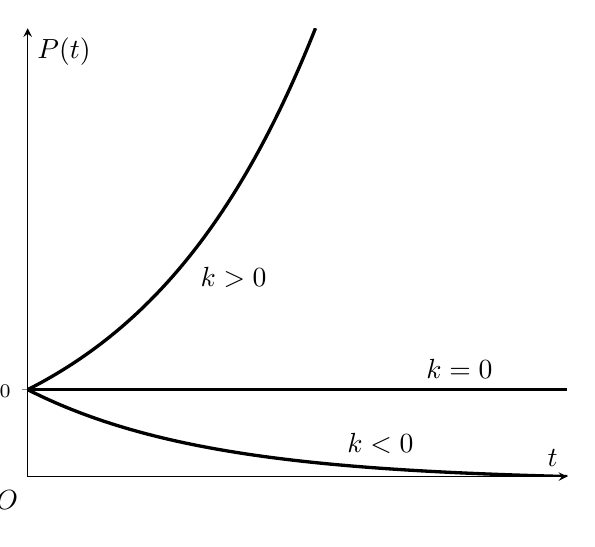
\begin{tikzpicture}[trim axis left, trim axis right]
        \begin{axis}[
            domain = 0:3,
            restrict y to domain = 0:5,
            samples = 101,
            axis y line=middle,
            axis x line=middle,
            xtick = \empty,
            ytick = {1},
            yticklabels = {$p_0$},
            xlabel = {$t$},
            ylabel = {$P(t)$},
            legend cell align={left},
            legend pos=outer north east,
            after end axis/.code={
                \path (axis cs:0,0) 
                    node [anchor=north east] {$O$};
                }
            ]
            \addplot[very thick, domain=0:2] {e^(x)} node[pos=0.4, below right] {$k > 0$};

            \addplot[very thick] {1} node[pos=0.8, above] {$k = 0$};

            \addplot[very thick] {e^(-x)} node[pos=0.6, above right] {$k < 0$};
            \end{axis}
    \end{tikzpicture}
    \caption{}
\end{figure}

While the cases where $k \leq 0$ are possible to happen in real life, the case where $k > 0$ is not realistically possible as most populations are constrained by limitations of resources.

\subsection{Logistic Growth Model}

To make the exponential model more realistic when $k > 0$, we can cap the population at some constant $N$. That is, when the population is small relative to $N$, the population grows exponentially, but as it approaches the population cap $N$, its growth rate approaches 0.

We may account for the growth rate declining to 0 by including a factor of $1 - P/N$ in the exponential model. This is because $1 - P/N$ is close to 1 (i.e. no effect) when $P \ll N$, and close to 0 when $P \approx N$. The resulting model \[\der{P}{t} = kP\bp{1 - \frac{P}{N}},\] is called the \vocab{logistic growth model}. $k$ is called the \vocab{intrinsic growth rate}, while $N$ is called the \vocab{carrying capacity}.

Given the initial condition $P(0) = p_0$, the solution of the logistic equation is \[P(t) = \frac{p_0 N}{p_0 + (N-p_0) \e^{-kt}}.\]

\begin{figure}[H]\tikzsetnextfilename{375}
    \centering
    \begin{tikzpicture}[trim axis left, trim axis right]
        \begin{axis}[
            domain = 0:7,
            restrict y to domain =0:5,
            samples = 101,
            axis y line=middle,
            axis x line=middle,
            ymin = 0,
            xtick = \empty,
            ytick = {4, 1},
            yticklabels = {$N$, $p_0$},
            ymax = 6,
            xlabel = {$t$},
            ylabel = {$P(t)$},
            legend cell align={left},
            legend pos=outer north east,
            after end axis/.code={
                \path (axis cs:0,0) 
                    node [anchor=north east] {$O$};
                }
            ]
            \addplot[very thick] {4/(1 + 3 * e^(-x))};
            \addplot[dashed] {4};
            \end{axis}
    \end{tikzpicture}
    \caption{}
\end{figure}

\subsubsection{Long-Term Behaviour}

We now analyse the long-term behaviour of the model, which is determined by the value of $p_0$.

Notice that the derivative of the logistic growth model, $\derx{P}{t} = kP(1 - P/N)$, is 0 at $P = 0$ and $P = N$. Also notice that these are also solutions to the differential equation. These two values are the \vocab{equilibrium points} since they are constant solutions to the differential equation.

Consider the case where $k > 0$.

\begin{figure}[H]\tikzsetnextfilename{376}
    \centering
    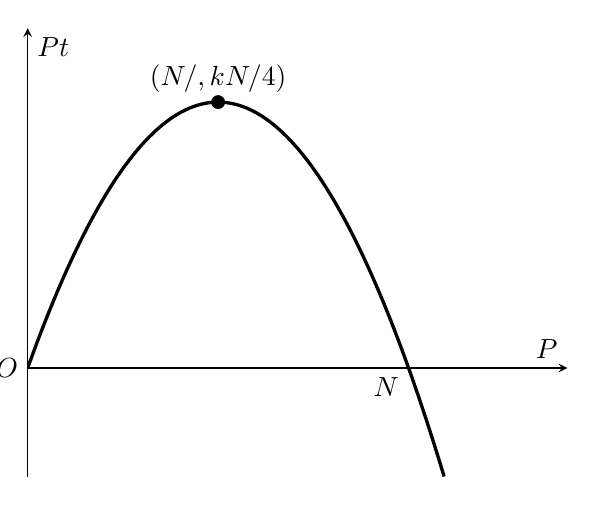
\begin{tikzpicture}[trim axis left, trim axis right]
        \begin{axis}[
            domain = 0:8,
            restrict y to domain=-4:11.5,
            xmax=8.5,
            samples = 101,
            axis y line=middle,
            axis x line=middle,
            xtick = \empty,
            ytick = \empty,
            ymax = 11.5,
            xlabel = {$P$},
            ylabel = {$\derx{P}{t}$},
            legend cell align={left},
            legend pos=outer north east,
            after end axis/.code={
                \path (axis cs:0,0) 
                    node [anchor=east] {$O$};
                }
            ]
            \addplot[very thick] {x * (6 - x)};
            \node[anchor=north east] at (6, 0) {$N$};

            \fill (3, 9) circle[radius=2.5pt] node[anchor=south] {$(N/, k N/4)$};
            \end{axis}
    \end{tikzpicture}
    \caption{}
\end{figure}

From the above diagram, we observe that
\begin{itemize}
    \item if $0 < p_0 < N$, then $P$ will increase towards $N$ since $\derx{P}{t} > 0$.
    \item if $p_0 > N$, then $P$ will decrease towards $N$ since $\derx{P}{t} < 0$.
\end{itemize}

Since any population value in the neighbourhood of 0 will move away from 0, the equilibrium point at $P = 0$ is known as an \vocab{unstable equilibrium point}. On the contrary, since any population value in the neighbourhood of $N$ will move towards $N$, the equilibrium point at $P = N$ is known as a \vocab{stable equilibrium point}.

Now consider the case where $k < 0$.

\begin{figure}[H]\tikzsetnextfilename{377}
    \centering
    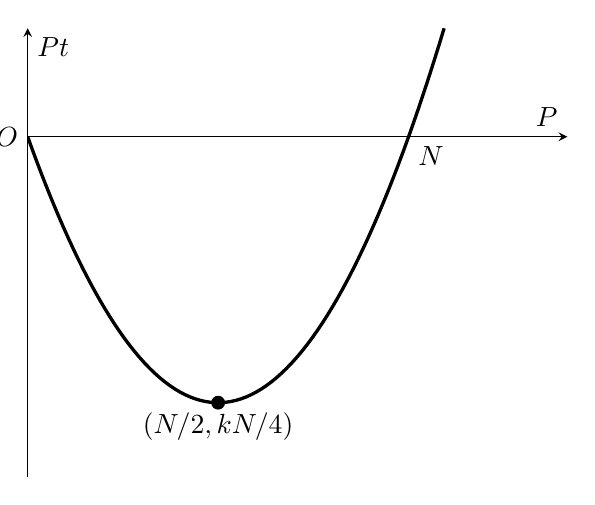
\begin{tikzpicture}[trim axis left, trim axis right]
        \begin{axis}[
            domain = 0:8,
            xmax=8.5,
            restrict y to domain=-11.5:4,
            samples = 101,
            axis y line=middle,
            axis x line=middle,
            xtick = \empty,
            ytick = \empty,
            ymin = -11.5,
            xlabel = {$P$},
            ylabel = {$\derx{P}{t}$},
            legend cell align={left},
            legend pos=outer north east,
            after end axis/.code={
                \path (axis cs:0,0) 
                    node [anchor=east] {$O$};
                }
            ]
            \addplot[very thick] {-x * (6 - x)};
            \node[anchor=north west] at (6, 0) {$N$};

            \fill (3, -9) circle[radius=2.5pt] node[anchor=north] {$(N/2, k N/4)$};
            \end{axis}
    \end{tikzpicture}
    \caption{}
\end{figure}

From the above diagram, we observe that
\begin{itemize}
    \item if $0 < p_0 < N$, then $P$ will decrease towards $N$ since $\derx{P}{t} < 0$.
    \item if $p_0 > N$, then $P$ will increase indefinitely since $\derx{P}{t} > 0$.
\end{itemize}

In this case, the equilibrium point at $P = 0$ is stable, while the equilibrium point at $P = N$ is unstable.

Thus, we see that what happens to the population in the long-run depends very much on the value of the initial population, $p_0$.

\subsection{Harvesting}

There are many single population systems for which harvesting takes place. \vocab{Harvesting} is a removal of a certain number of the population during each time period that the harvesting takes place. Below are some variants of the basic logistic model.

\subsubsection{Constant Harvesting}

The most direct way of harvesting is to use a strategy where a constant number, $H \geq 0$, of individuals are removed during each time period. For this situation, the logistic equation gets modified to the form \[\der{P}{t} = kP\bp{1 - \frac{P}{N}} - H,\] where $H$ is known as the \vocab{harvesting rate}.

Observe that the equilibrium solutions to this modified logistic equation are: \[P = \frac{N}{2} \pm \sqrt{\frac{N^2}{4} - \frac{NH}{k}}.\] With the equilibrium solutions, we can do the same analysis as we did with the logistic model to determine the long-term behaviour of this model.

\subsubsection{Variable Harvesting}

The model \[\der{P}{t} = kP \bp{1 - \frac{P}{N}} - HP\] results by harvesting at a non-constant rate proportional to the present population $P$. The effect is to decrease the natural growth rate $k$ by a constant amount $H$ in the standard logistic model.

\subsubsection{Restocking}

The equation \[\der{P}{t} = kP \bp{1 - \frac{P}{N}} - H \sin{\o t}\] models a logistic equation that is periodically harvested and restocked with maximal rate $H$. For sufficiently large $p_0$, the equation models a stable population that oscillates about the carrying capacity $N$ with period $T = 2\pi / \o$.